\chapter{Arhitektura i dizajn sustava} \label{arhitektura}
		
%		\textbf{\textit{dio 1. revizije}}\\
		
%		\textit{ Potrebno je opisati stil arhitekture te identificirati: podsustave, preslikavanje na radnu platformu, spremišta podataka, mrežne protokole, globalni upravljački tok i sklopovsko-programske zahtjeve. Po točkama razraditi i popratiti odgovarajućim skicama:}

%	\begin{itemize}
%		\item 	\textit{izbor arhitekture temeljem principa oblikovanja pokazanih na predavanjima (objasniti zašto ste baš odabrali takvu arhitekturu)}
%		\item 	\textit{organizaciju sustava s najviše razine apstrakcije (npr. klijent-poslužitelj, baza podataka, datotečni sustav, grafičko sučelje)}
%		\item 	\textit{organizaciju aplikacije (npr. slojevi frontend i backend, MVC arhitektura) }		
%	\end{itemize}



%   OVDJE PIŠE ŠTO TREBA NAPISATI!---^^^
		
    \noindent { Arhitektura se može podijeliti na tri podsustava:}
	\begin{itemize}
		\item{Web poslužitelj}
		\item{Web aplikacija}
		\item{Baza podataka}		
	\end{itemize}
	
	\underline{\textit{Web poslužitelj}} osnova je rada web aplikacije. Njegova primarna zadaća je komunikacija klijenta s aplikacijom. Komunikacija se odvija preko HTTP (engl. Hyper Text Transfer Protocol) protokola, što je protokol u prijenosu informacija na webu. Poslužitelj je onaj koji pokreće web aplikaciju te joj prosljeđuje zahtjev.
	
	Korisnik koristi \underline{\textit{web aplikaciju}} za obrađivanje željenih zahtijeva. Web aplikacija obrađuje zahtjev te ovisno o zahtjevu, pristupa bazi podataka, vraća web-poslužitelju odgovor u JSON formatu, a zatim web poslužitelj te informacije prikazuje na svoj način.
		\begin{figure}[H]
                    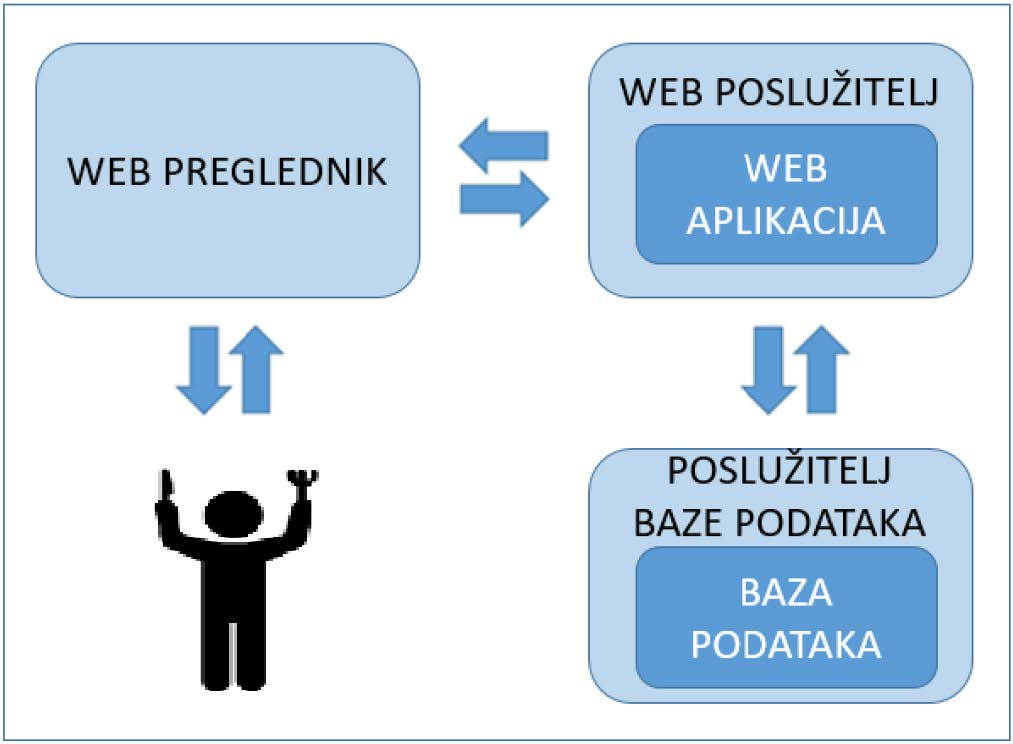
\includegraphics[scale=1]{slike/Arhitektura sustava.jpg}
        			\centering
        			\caption{Arhitektura sustava}
        			\label{fig:arhitekturaSustava}
        		\end{figure}
			
			\eject

	Programski jezik koji smo odabrali za izradu naše web aplikacije je Java zajedno sa SpringBoot radnim okvirom te programski jezik Javascript s React bibliotekom (eng. library). Odabrano razvojno okruženje je IntelliJ. 
	
	Arhitektura sustava sastoji se od 3 razine:
	\begin{itemize}
		\item{\textbf{Sučelje} - Najviša razina aplikacije, glavna funkcija sučelja je prevesti procese i rezultate u format koji korisnik može razumijeti}
		\item{\textbf{Logika} - Ova razina koordinira aplikaciju, obrađuje naredbe, izvršava logiku i računa. Također prenosi podatke između podatkovne razine i sučelja.}
		\item{\textbf{Podatci} - Ova razina uključuje spremanje i dohvaćanje podatke iz baze podataka}		
	\end{itemize}
	
	Funkcionalnosti aplikacije se izvršavaju slanjem upita na \textit{\underline{endpointe}}. Oni definiraju adresu ili točku spajanja na Web poslužitelj. Tipično je reprezentiran jednostavnim HTTP URL-om (adresom, \textit{linkom}).
	
	Implementirani Endpointi su:
	\begin{itemize}
	    \item {\textbf{Prijava} - Omogućava pristup korisničkom računu, provjerava jeli dobro postavljen session cookie}
	    \item {\textbf{Kreiranje donora od strane donora}}
	    \item {\textbf{Kreiranje donora od strane radnika}}
	    \item {\textbf{Prikaz korisničkih podataka}}
	\end{itemize}

	

	
		

		

				
		\section{Baza podataka}
			
%			\textbf{\textit{dio 1. revizije}}\\
			
		Sustav koristi relacijsku bazu podataka. Relacijske baze podataka pohranjuju i pružaju pristup podatcima. Gradivna jedinka baze je relacija, odnosno tablica koja je definirana svojim imenom i skupom atributa. Prednost relacijskih baza jest lakše definiranje odnosa između podataka. Baza podataka ove aplikacije sastoji se od ovih entiteta:
		\begin{itemize}
	        \item Korisnik
	        
	        \begin{itemize}
	            \item Donor krvi
	            \item Djelatnik banke
	        \end{itemize}
	        
	        \item Zaliha krvi
	        \item Pokušaj donacije
	        
	        
	    \end{itemize}
		
		
			\subsection{Opis tablica}
			

		%		\textit{Svaku tablicu je potrebno opisati po zadanom predlošku. Lijevo se nalazi točno ime varijable u bazi podataka, u sredini se nalazi tip podataka, a desno se nalazi opis varijable. Svjetlo zelenom bojom označen je primarni ključ. Svjetlo plavom označen je strani ključ. Svijetlo tirkiznom bojom označen je ključ koji je primarni i strani. Svijetlo crvenom bojom označeni su unique atributi koji nisu ključevi.}
				
				
				
				
			% OVO STAVI KAO NASLOV SVAKE TABLICE U OVE PRVE UGLATE ZAGRADE, GDJE PIŠE LABEL=NONE (mozes vidjeti primjer kod dnevnika promjena)
			%caption = {Dnevnik promjena dokumentacije}
			
		\textbf{Korisnik} - Ovaj entitet sadržava sve administrativne podatke o korisniku aplikacije, njegovi osnovni podatci nalaze se u drugim, personiliziranim entitetima. Sadrži atribute: user id, user role, password, acc activated, perm deactivated, opt out. Ovaj entitet u vezi je \textit{One-to-one} sa entitetima Donorom i Djelatnikom banke preko atributa donor id, odnosno bank worker id. 
			
				\begin{longtblr}[
				    caption = {Tablica \textit{korisnik} u bazi podataka},
					label=none
					]{
						width = \textwidth,
						colspec={|X[6,l]|X[7, l]|X[20, l]|}, 
						rowhead = 1,
					} %definicija širine tablice, širine stupaca, poravnanje i broja redaka naslova tablice
					\hline \multicolumn{3}{|c|}{\textbf{Korisnik}}	 \\ \hline[3pt]
					\SetCell{LightGreen}user id & BIGINT	&  	Jedinstveni identifikator korisnika  	\\ \hline
					user role	& VARCHAR(20) &  Je li korisnik donor, djelatnik  banke ili administrator 	\\ \hline 
					password & VARCHAR(128) &  Enkriptirana lozinka korisnika \\ \hline 
					acc activated & INT	& Je li korisnik preko e-maila aktivirao svoj račun  		\\ \hline 
					perm deactivated & INT &  Je li korisnički račun trajno dekativiran \\ \hline 
					opt out & INT &  Je li uključena opcija koja isključuje notifikacije \\ \hline 
				\end{longtblr}
				
				
		\textbf{Donor} - Ovaj entitet sadržava osobne podatke o korisniku aplikacije koji je donor. Sadrži atribute: donor id, first name, last name, oib, birth date, birth place, address, work place, private contact, work contact, email, blood type. Ovaj entitet u vezi je \textit{One-to-many} sa entitetom Pokušaj donacije preko atributa donor id. Također je u vezi \textit{One-to-one} sa entitetom Korisnik preko atributa donor id.
				
				\begin{longtblr}[
				    caption = {Tablica \textit{donor} u bazi podataka},
					label=none
					]{
						width = \textwidth,
						colspec={|X[6,l]|X[7, l]|X[20, l]|}, 
						rowhead = 1,
					} %definicija širine tablice, širine stupaca, poravnanje i broja redaka naslova tablice
					\hline \multicolumn{3}{|c|}{\textbf{Donor}}	 \\ \hline[3pt]
					\SetCell{LightTeal}donor id & BIGINT	&  	Jedinstveni identifikator donora krvi, odgovara identifikatoru korisnika  	\\ \hline
					first name	& VARCHAR(50) &  Ime donora krvi 	\\ \hline 
					last name & VARCHAR(50) &  Prezime donora krvi \\ \hline 
					\SetCell{LightRed}oib & CHAR(11)	& OIB donora krvi  		\\ \hline 
					birth date & DATE &  Datum rođenja donora krvi \\ \hline 
					birth place & VARCHAR(100) &  Mjesto rođenja donora krvi \\ \hline 
					address & VARCHAR(100)	& Adresa stanovanja donora krvi  		\\ \hline 
					work place & VARCHAR(100) &  Mjesto zaposlenja donora krvi \\ \hline 
					private contact & VARCHAR(20) &  Osobni kontakt broj mobitela donora krvi \\ \hline 
					work contact & VARCHAR(20) &  Poslovni kontakt broj mobitela donora krvi \\ \hline 
					email & VARCHAR(50) &  e-mail adresa donora krvi \\ \hline 
					\SetCell{LightBlue}blood type & VARCHAR(3) &  Krvna grupa donora krvi \\ \hline 
					perm rejected reason & VARCHAR(100) &  Ako je račun donora krvi trajno deaktiviran, razlog deaktivacije \\ \hline
				\end{longtblr}
				
		\textbf{Djelatnik banke} - Ovaj entitet sadržava osobne podatke djelatnika banke. Sadrži atribute: bank worker id, first name, last name, oib, birth date, birth place, address, work place, private contact, work contact, email. U vezi je \textit{One-to-one} sa entitetom Korisnik preko atributa bank worker id.
				
				\begin{longtblr}[
				    caption = {Tablica \textit{djelatnik banke} u bazi podataka},
					label=none
					]{
						width = \textwidth,
						colspec={|X[6,l]|X[7, l]|X[20, l]|}, 
						rowhead = 1,
					} %definicija širine tablice, širine stupaca, poravnanje i broja redaka naslova tablice
					\hline \multicolumn{3}{|c|}{\textbf{Djelatnik banke}}	 \\ \hline[3pt]
					\SetCell{LightTeal}bank worker id & BIGINT	&  	Jedinstveni identifikator djelatnika banke, odgovara identifikatoru korisnika  	\\ \hline
					first name	& VARCHAR(50) &  Ime djelatnika banke  	\\ \hline 
					last name & VARCHAR(50) &  Prezime djelatnika banke  \\ \hline 
					\SetCell{LightRed}oib & CHAR(11)	& OIB djelatnika banke   		\\ \hline 
					birth date & DATE &  Datum rođenja djelatnika banke  \\ \hline 
					birth place & VARCHAR(100) &  Mjesto rođenja djelatnika banke  \\ \hline 
					address & VARCHAR(100)	& Adresa stanovanja djelatnika banke  		\\ \hline 
					work place & VARCHAR(100) &  Mjesto zaposlenja djelatnika banke  \\ \hline 
					private contact & VARCHAR(20) &  Osobni kontakt broj mobitela djelatnika banke  \\ \hline
					work contact & VARCHAR(20) &  Poslovni kontakt broj mobitela djelatnika banke  \\ \hline 
					email & VARCHAR(50) &  e-mail adresa djelatnika banke  \\ \hline 
				\end{longtblr}
				
		\textbf{Zaliha krvi} - Ovaj entitet sadržava podatke o količini krvi u banci. Sadrži atribute: number of units, max units, min units.
			
				\begin{longtblr}[
				    caption = {Tablica \textit{zaliha krvi} u bazi podataka},
					label=none
					]{
						width = \textwidth,
						colspec={|X[6,l]|X[6, l]|X[20, l]|}, 
						rowhead = 1,
					} %definicija širine tablice, širine stupaca, poravnanje i broja redaka naslova tablice
					\hline \multicolumn{3}{|c|}{\textbf{Zaliha krvi}}	 \\ \hline[3pt]
					\SetCell{LightGreen}blood type & CHAR(3) & Krvna grupa jedinice krvi \\ \hline
					number of units	& INT &  Trenutni broj jedinica krvi  	\\ \hline 
					max units & INT &  Maksimalni broj jedinica krvi \\ \hline 
					min units & INT	& Minimalni broj jedinica krvi \\ \hline 
				\end{longtblr}
				
		\textbf{Pokušaj donacije} - Ovaj entitet sadržava podatke o pojedinoj donaciji krvi. Sadrži atribute: donation id, rejected reason, blood type, donor id, bank worker id. U vezi je \textit{Many-to-one} sa entitetom Donor preko atributa donor id.
		        
				\begin{longtblr}[
				    caption = {Tablica \textit{pokušaj donacije} u bazi podataka},
					label=none
					]{
						width = \textwidth,
						colspec={|X[6,l]|X[7, l]|X[20, l]|}, 
						rowhead = 1,
					} %definicija širine tablice, širine stupaca, poravnanje i broja redaka naslova tablice
					\hline \multicolumn{3}{|c|}{\textbf{Pokušaj donacije}}	 \\ \hline[3pt]
					rejected reason	& VARCHAR(100) &  Razlog neuspješnosti pokušaja darivanja krvi 	\\ \hline 
					\SetCell{LightBlue}blood type & CHAR(3) &  Kvrna grupa donora krvi koji obavlja ovu donaciju \\ \hline 
					\SetCell{LightBlue}donor id & BIGINT	& Jedinstveni identifikator donora krvi koji obavlja ovu donaciju krvi \\ \hline 
					\SetCell{LightBlue}bank worker id & BIGINT	& Jedinstveni identifikator djelatnika banke koji nadgleda ovu donaciju krvi \\ \hline 
				\end{longtblr}
				
				
			
			\subsection{Dijagram baze podataka}
			
				
				\begin{figure}[H]
                    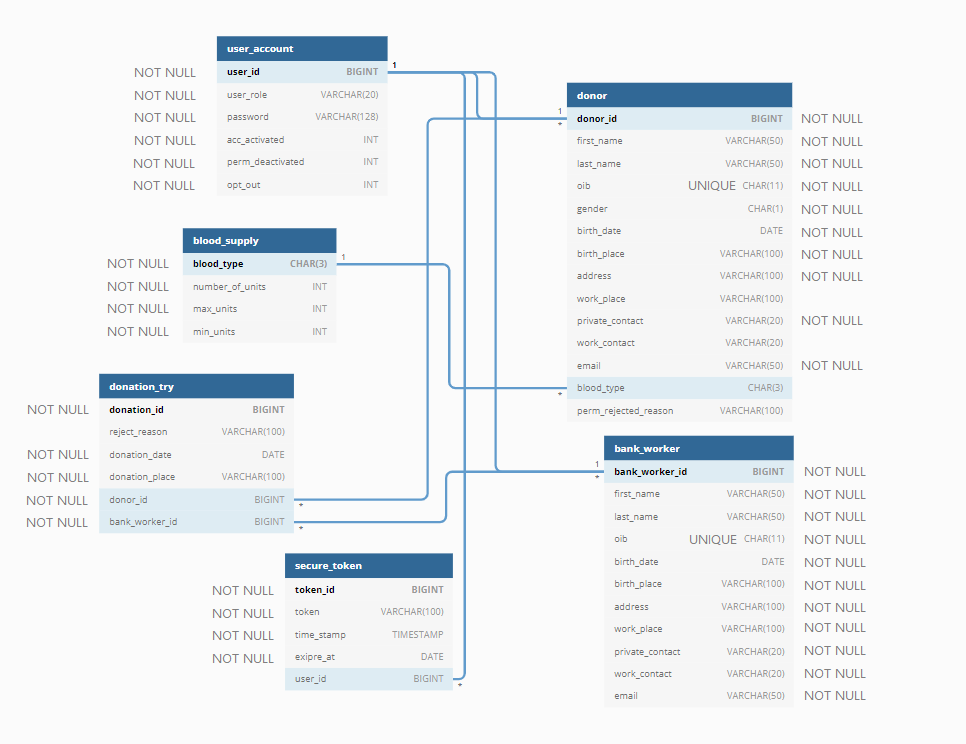
\includegraphics[scale=0.7]{slike/DB DIAGRAM.png}
        			\centering
        			\caption{Dijagram baze podataka}
        			\label{fig:dbDiagram}
        		\end{figure}
			
			\eject
			
			
		\section{Dijagram razreda}
		
%			\textit{Potrebno je priložiti dijagram razreda s pripadajućim opisom. Zbog preglednosti je moguće dijagram razlomiti na više njih, ali moraju biti grupirani prema sličnim razinama apstrakcije i srodnim funkcionalnostima.}\\
			
%			\textbf{\textit{dio 1. revizije}}\\
			
%			\textit{Prilikom prve predaje projekta, potrebno je priložiti potpuno razrađen dijagram razreda vezan uz \textbf{generičku funkcionalnost} sustava. Ostale funkcionalnosti trebaju biti idejno razrađene u dijagramu sa sljedećim komponentama: nazivi razreda, nazivi metoda i vrste pristupa metodama (npr. javni, zaštićeni), nazivi atributa razreda, veze i odnosi između razreda.}\\

    Na slikama u nastavku prikazani su razredi koji pripadaju arhitekturi poslužiteljske aplikacije. Radi preglednosti, dijagram razreda razlomljen je na više njih, grupiranih prema sličnim razinama apstrakcije i srodnim funkcionalnostima.
                \begin{figure}[H]
                    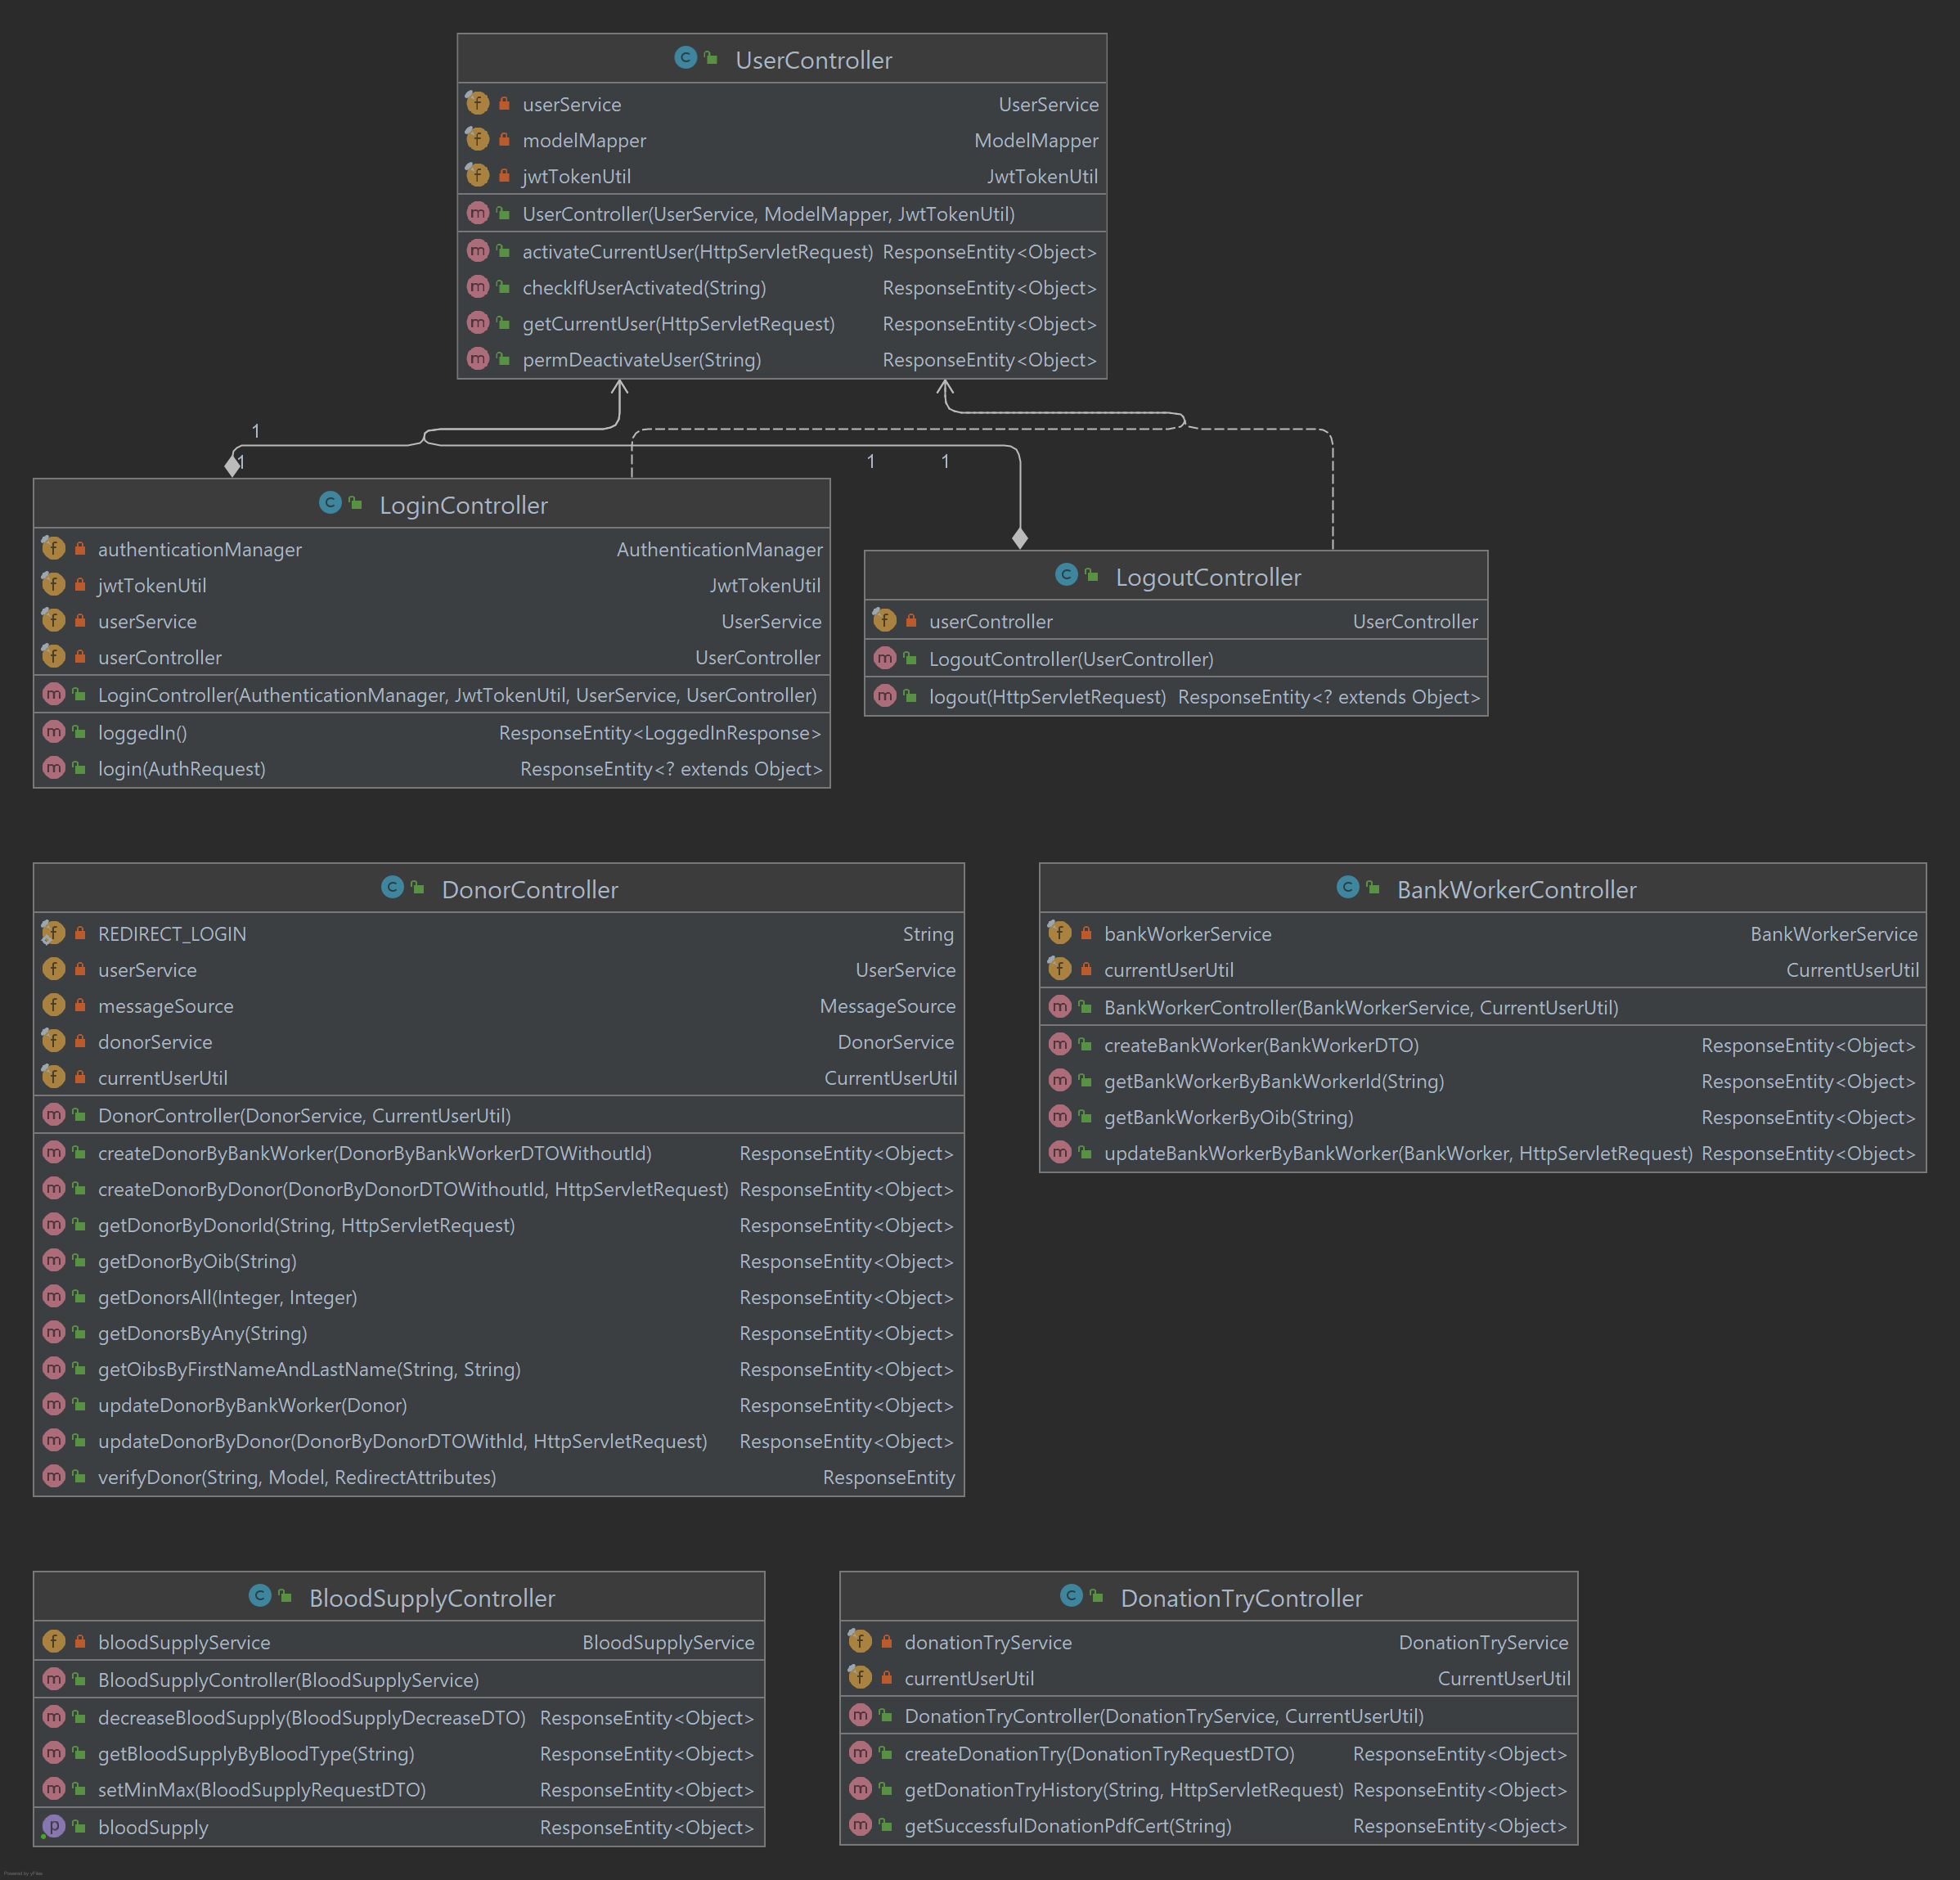
\includegraphics[scale=0.20]{slike/Controller.png}
        			\centering
        			\caption{Dijagram controller klasa}
        			\label{fig:controller}
        		\end{figure}
    \textbf{\textit{Controller}} klase vraćaju entitet odgovora (\textit{response entity}) kao odgovor na zahtjeve na krajnje točke. Entitet odgovora je objekt koji sadrži HTTP status i JSON (\textit{JavaScript Object Notation}) podatke. Obično se radi o dohvaćanju podataka koje korisnik aplikacije zahtjeva. U \textit{Controller} klasama je također određeno kojim krajnjim točkama korisnici imaju pristup (ovisno o ulozi korisnika) pomoću anotacija. Metode u Controller klasama obično pozivaju metode istog imena u odgovarajućim Service klasama te ih se može shvatiti kao klase koje svoju funkcionalnost vrše koristeći poslovnu logiku iz Service klasa. Ako neki Controller sadrži objekt tipa Service (većina ih sadrži), tada on koristi neke od metoda iz odgovarajuće Service klase. Bitno je napomenuti da se koristi @Controller notacija.
    
    \textbf{LoginController} zadužen je za ostvarivanje funkcionalnosti prijave. Login prima HTTP GET zahtjev. Koristi se osnovna autentikacija (\textit{basic authentication}), što znači da su u autorizacijskom zaglavlju (\textit{Authorization header}) zapisani userId i lozinka. Provjerava se postoji li u sustavu korisnik s navedenim identifikacijskim brojem, te ako postoji provjeriti je li lozinka u zahtjevu jednaka onoj zapisanoj u bazi. Lozinke se spremaju i provjeravaju u kodiranom obliku pomoću \textit{BCryptEncodera}. Kod vraćanja odgovora postavlja se kolačić sa sjednicom (\textit{session cookie}), a ukoliko su navedeni podaci ispravni, zapisuju se podatci o prijavljenom korisniku (poput imena i uloga). Ukoliko podaci nisu ispravni vraća se kod o pogrešci 401. Uz naredne zahtjeve korisnika prilaže se kolačić sa sjednicom čime poslužiteljska strana može prepoznati korisnikovu sjednicu i potvrditi da je korisnik prijavljen.
    
    \textbf{UserController} služi za: 
    \begin{itemize}
        \item Aktivaciju korisnika i provjeru stanja aktiviranosti korisnika
        \item Dohvaćanje korisnika
        \item Trajnu deaktivaciju korisničkog računa.
    \end{itemize}
    
    \textbf{DonorController} služi za: 
    \begin{itemize}
        \item Dohvaćanje i kreiranje donora 
        \item Dohvaćanje OIB-a donora
        \item Upravljanje podatatcima donora
    \end{itemize}
    
    \textbf{DonationTryController} služi za: 
    \begin{itemize}
        \item Kreiranje pokušaja donacije
        \item Dohvaćanje povijesti pokušaja donacije
        \item Zahtjevanje pdf potvrde donacije
    \end{itemize}
    
    \textbf{BloodSupplyController} služi za: 
    \begin{itemize}
        \item Smanjivanje razine krvi
        \item Dohvaćanje pojedinačnih ili svih zaliha krvi (ovisno o krvnoj grupi)
        \item Postavljanje minimalne i maksimalne prihvatljive zalihe
    \end{itemize}
    
    \textbf{BankWorkerController} služi za: 
    \begin{itemize}
        \item Kreiranje, dohvaćanje i upravljanje djelatnikom banke
    \end{itemize}
    
    \begin{figure}[H]
        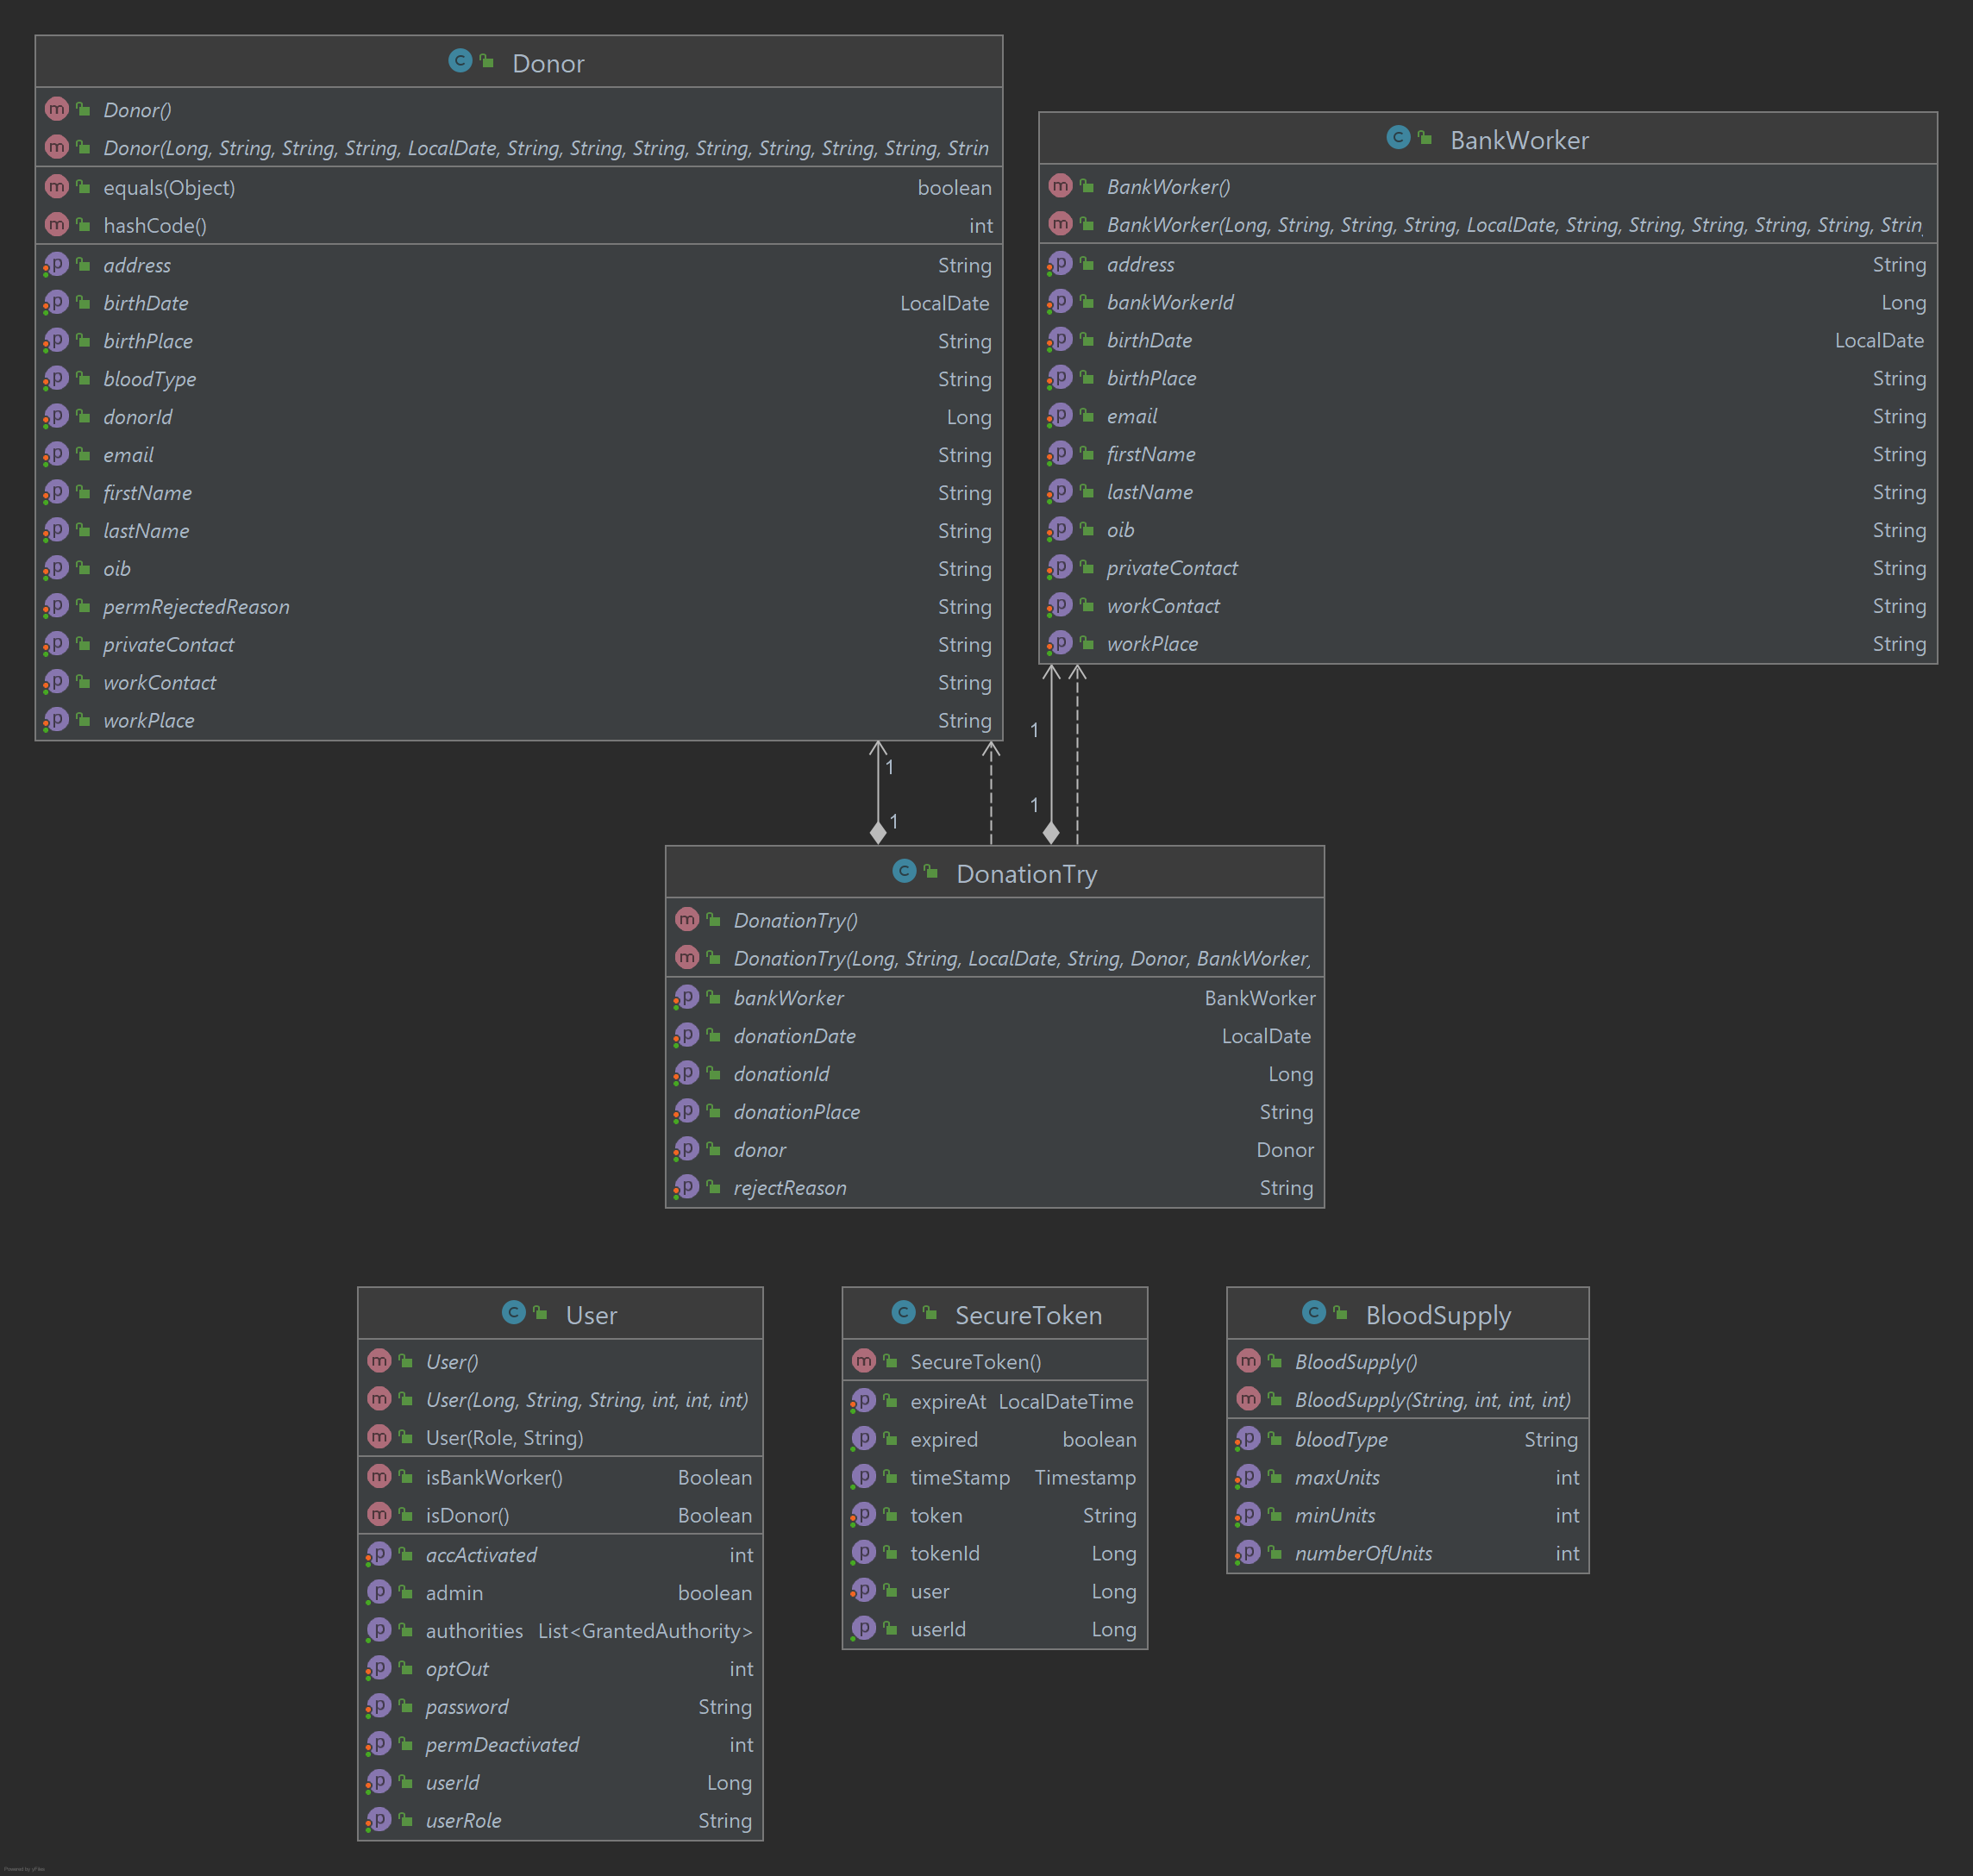
\includegraphics[scale=0.20]{slike/Model.png}
		\centering
		\caption{Dijagram model klasa}
		\label{fig:model}
    \end{figure}
    
    \textbf{\textit{Model}} klase služe za stvaranje objekata ekvivalentnim onima u bazi podataka. Ove klase ne sadrže metode koje obavljaju poslovnu logiku (samo gettere, settere, konstruktore itd.).  Valja navesti jednu iznimku, SecureToken model klasu, koja nema ekvivalent u bazi podataka. Taj objekt se koristi u svrhu generiranja jedinstvenoe poveznice. Više informacija nalazi se u opisu SecureTokenService klase. \textit{User}, \textit{Donor} i \textit{BankWorker} klase implementiraju sučelje \textit{Serializable}.
    
    \begin{figure}[H]
        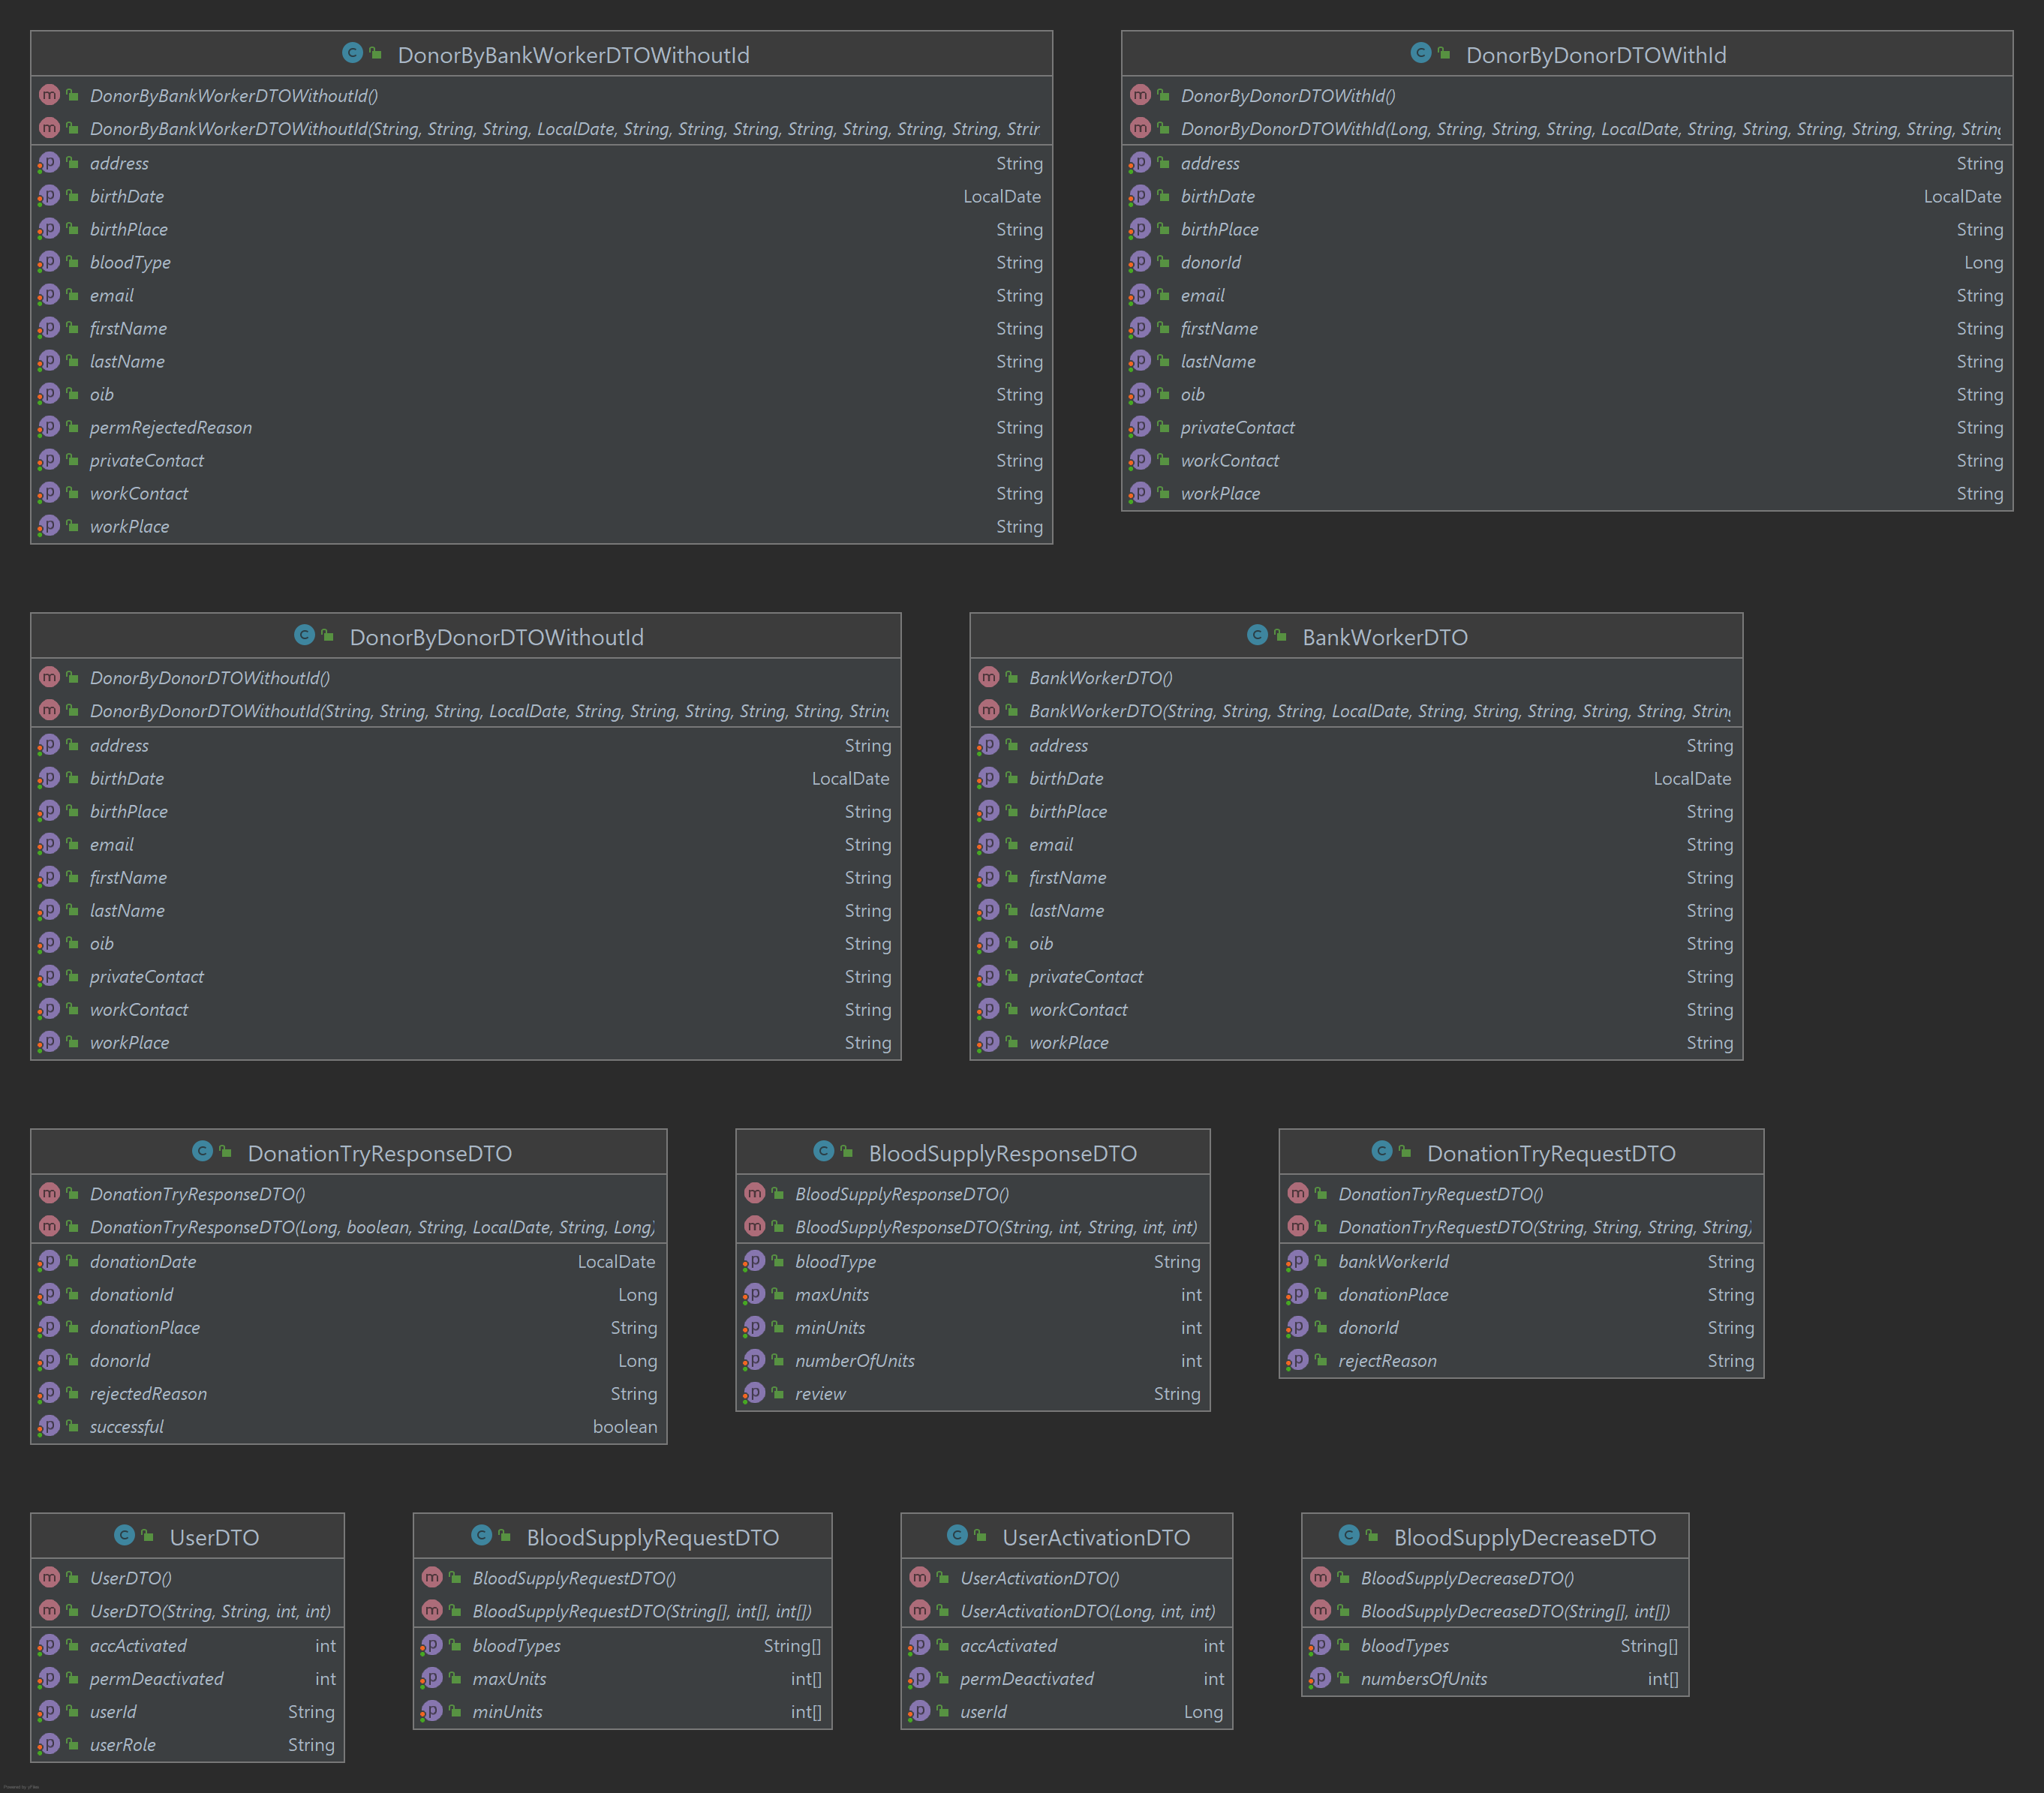
\includegraphics[scale=0.16]{slike/DTO.png}
		\centering
		\caption{Dijagram DTO klasa}
		\label{fig:DTO}
    \end{figure}
    \textbf{\textit{DTO}} (Data transfer object) klase služe kako bi se mogle vratiti na krajnje točke, i time izbjeći nepotrebno (ili nesigurno) slanje informacija koje nisu potrebne.
    
    
    \begin{figure}[H]
        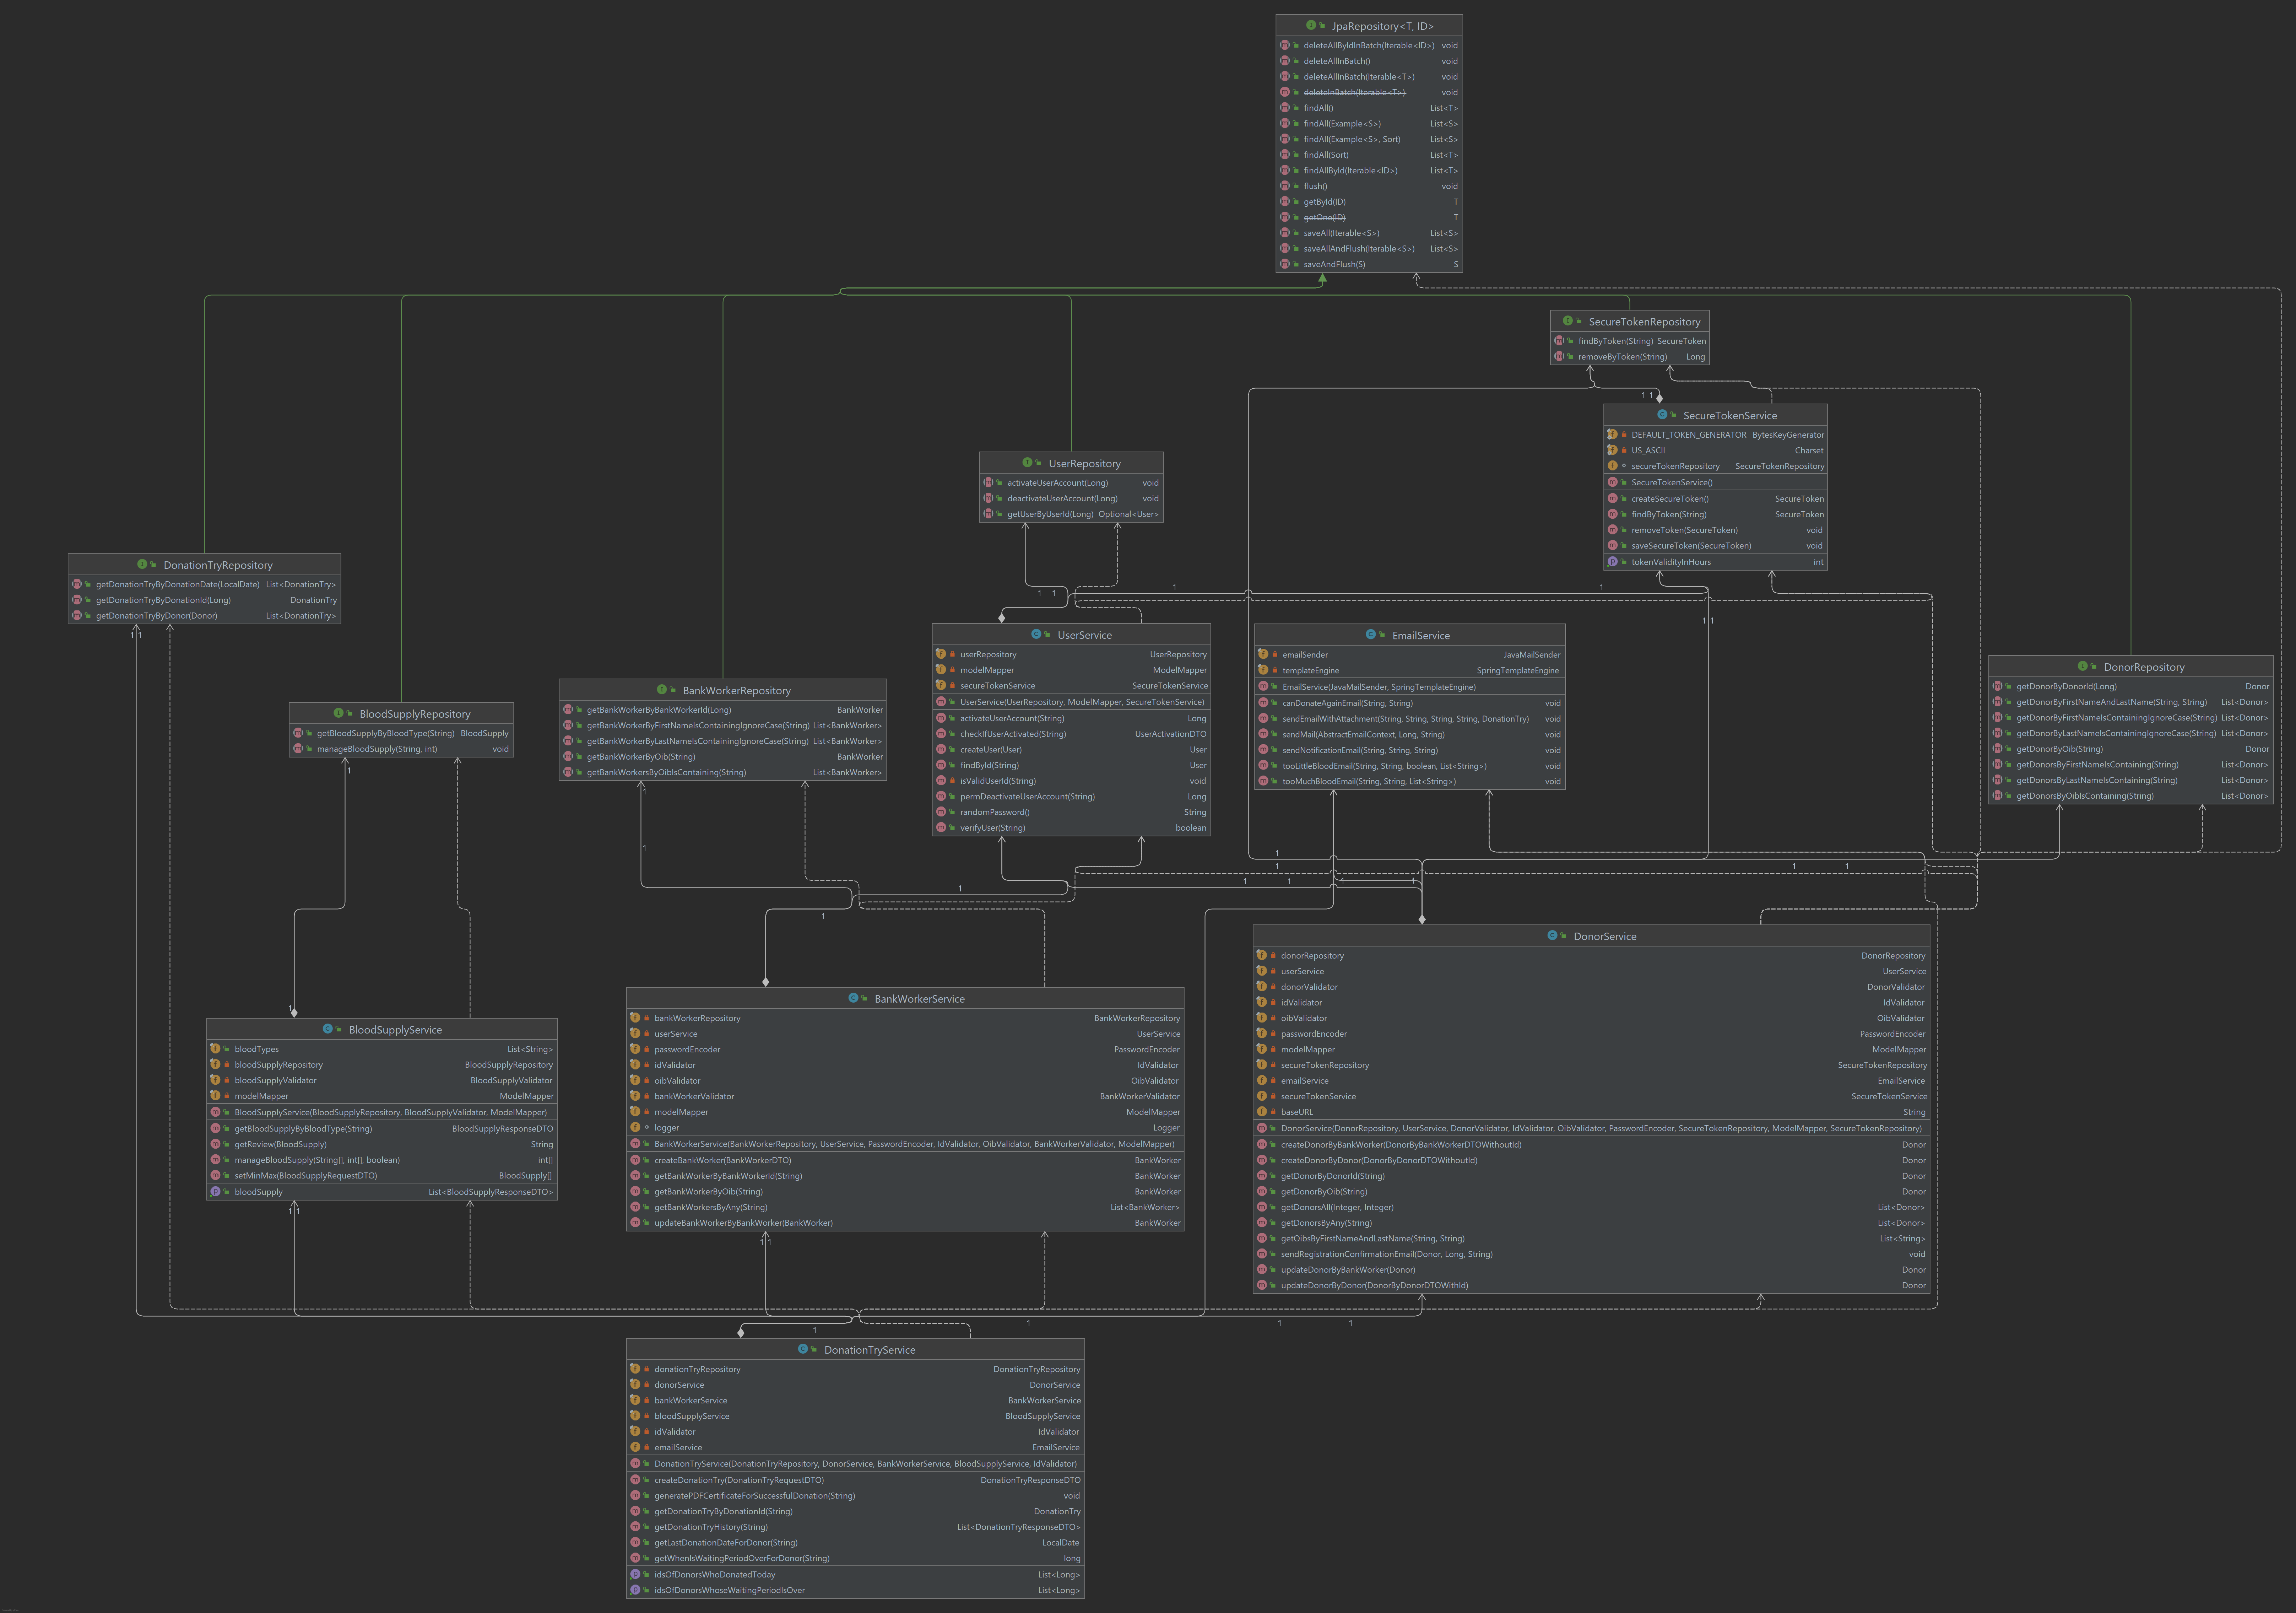
\includegraphics[scale=0.064]{slike/RepositoryService.png}
		\centering
		\caption{Dijagram Repository sučelja i Service klasa}
		\label{fig:repositoryService}
    \end{figure}
    
    Na sljedećoj poveznici nalazi se dijagram klasa za Repository i Service klase koji se može uvećati: \href{https://drive.google.com/file/d/1SzOhj1Bq-YyAUKqIZqTj0oUILVQYDE_b/view?usp=sharing}{\textcolor{blue}{Dijagram Repository sučelja i Service klasa}}
    
    
    \textbf{Repository} - Dohvaća i sprema podatke iz baze podataka, koristeći  sučelje \textit{JpaRepository}, koje sva Repository sučelja implementiraju. \textit{JpaRepository} je sučelje s metodama za pristup bazi podataka iz Spring-a, a metode se kreiraju same na temelju imenovanja metoda.
    
    \textbf{\textit{Service}} klase obavljaju poslovnu logiku aplikacije. Mnoge od metoda u Service klasama pozivaju su iz istoimenih metoda u odgovarajućim Controller klasama. Ako metode trebaju upravljati podatcima, koriste metode iz Repository sučelja.  Service klase uglavnom obavljaju logiku iza funkcionalnosti koje su navedene za Controller klase, ali valja navesti dvije iznimke:
    
    \textbf{EmailService} koji služi za slanje e-mailova (aktivacijskih i obavijesti) pomoću \textit{JavaMailSender} sučelja i
    \textbf{SecureTokenService} koji služi isključivo za generiranje jedninstvene poveznice koja se šalje u aktivacijskoj e-poruci. SecureTokenService u sebi sadrži objekt tipa \textit{BytesKeyGenerator} koji se koristi u spomenutom generiranju.
    
    \href{https://drive.google.com/file/d/1oA-XBPEW6Ks2GIoX5Iqn9XRFGumoSmCd/view?usp=sharing}{\textcolor{blue}{Dijagram svih klasa aplikacije}}-Na ovoj poveznici nalazi se dijagram svih klasa aplikacije.


			
			
%			\textbf{\textit{dio 2. revizije}}\\			
			
%			\textit{Prilikom druge predaje projekta dijagram razreda i opisi moraju odgovarati stvarnom stanju implementacije}
			
			
		    
		
		
\section{Dijagram stanja}
			
	\begin{figure}[H]
        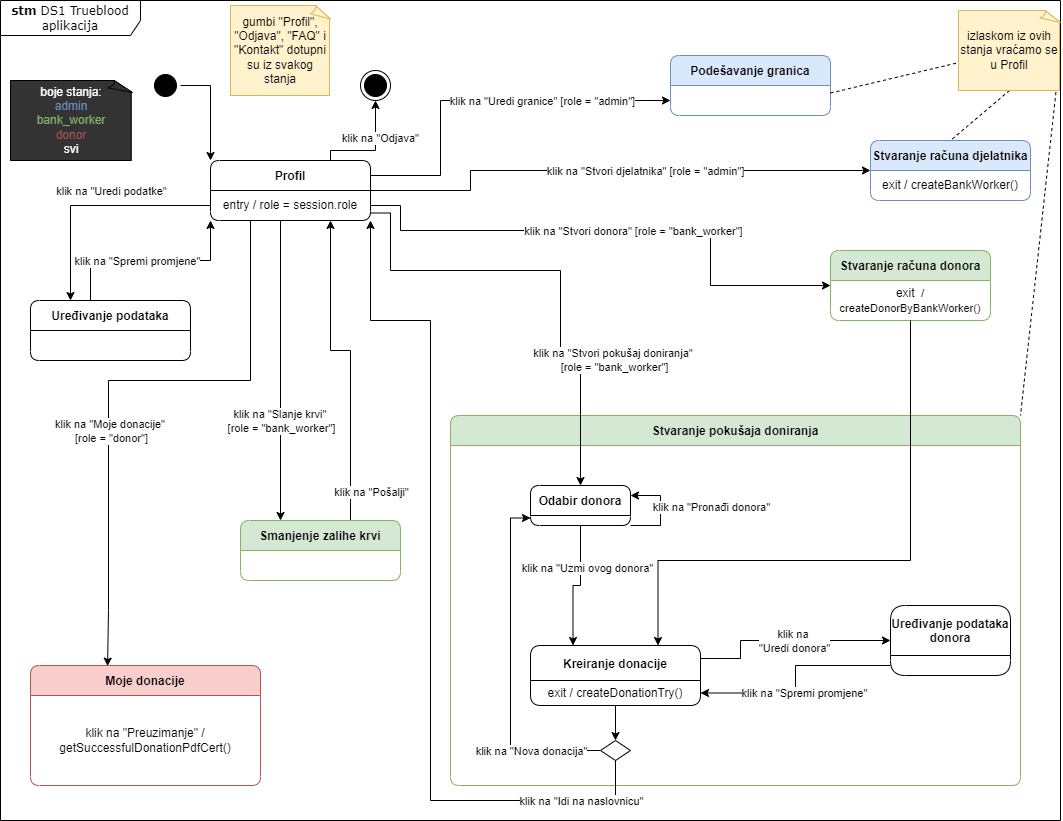
\includegraphics[scale=0.35]{slike/DS1_1.png}
    	\centering
    	\caption{DS1 Trueblood web aplikacija}
    	\label{fig:ds1}
    \end{figure}
    
    \par {
        \text Dijagram stanja prikazuje stanja u koje je moguće doći različitim akcijama korisnika. Stanja na dijagramu na slici 4.7 predstavljaju različite komponente Trueblood web aplikacije. Plavom bojom prikazane su komponente kojima može pristupiti administrator, zelenom djelatnik banke, crvenom donor, a bijelom svi. Sve funkcije navedene u dijagramu nalaze se u odgovarajućim \textit{controller} klasama. U početno stanje korisnik dolazi prijavom u sustav. Iz svakog stanja moguće se je odjaviti, doći u stanje profil te vidjeti često postavljana pitanja (FAQ) i kontakt, pritiskom na odgovarajuće gumbe. Iz stanja profil, korisnik može doći u razna druga stanja ovisno o svojoj ulozi. Svaki korisnik može urediti svoje podatke. Administrator ima mogućnost podešavanja optimalnih granica razina krvi u banci te može stvoriti račun djelatnika banke. Djelatnik banke ima mogućnost stvaranja računa donora, smanjivanja zaliha krvi te stvaranja pokušaja doniranja. Prilikom postupka doniranja, djelatnik banke može odabrati postojećeg donora ili stvoriti novog. Prema podacima donora djelatnik banke kreira donaciju koja se evidentira klikom na gumb "Doniraj".}

%			\textbf{\textit{dio 2. revizije}}\\
			
%			\textit{Potrebno je priložiti dijagram stanja i opisati ga. Dovoljan je jedan dijagram stanja koji prikazuje \textbf{značajan dio funkcionalnosti} sustava. Na primjer, stanja korisničkog sučelja i tijek korištenja neke ključne funkcionalnosti jesu značajan dio sustava, a registracija i prijava nisu. }
			
			

\section{Dijagram aktivnosti}

    \begin{figure}[H]
        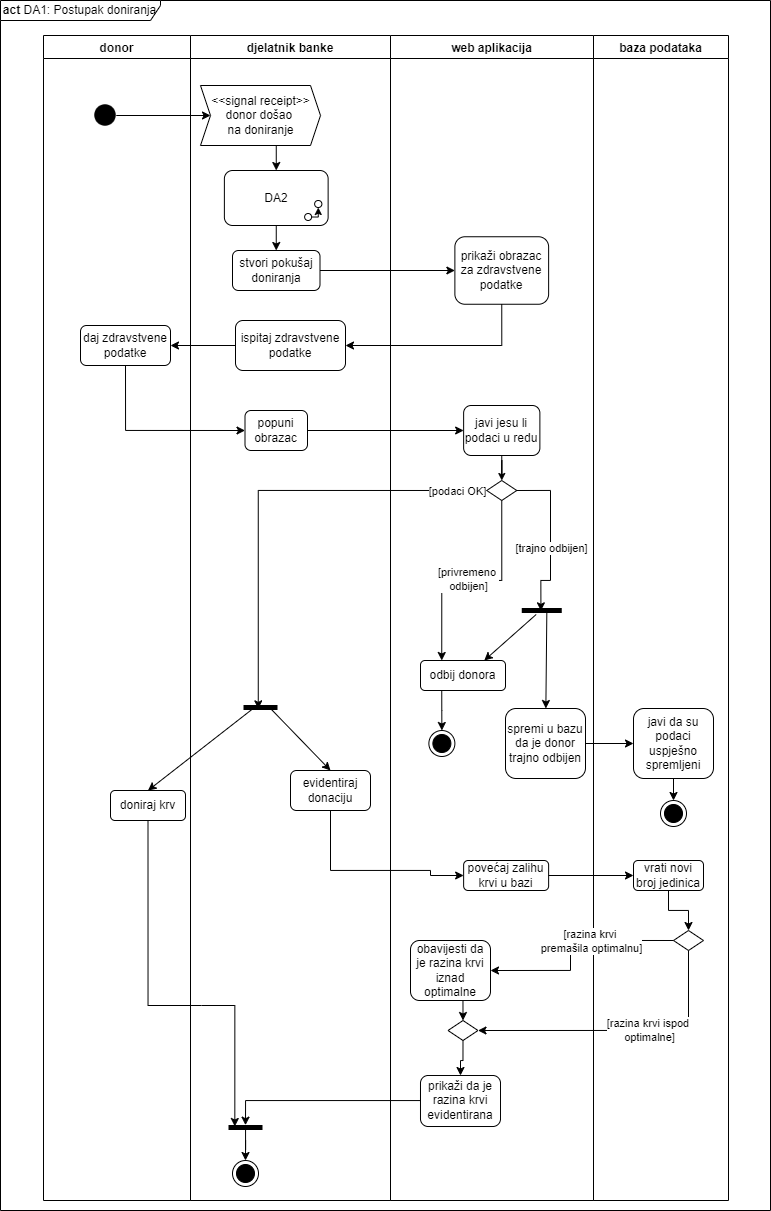
\includegraphics[scale=0.40]{slike/DA1 Postupak doniranja.png}
    	\centering
    	\caption{DA1 Postupak doniranja}
    	\label{fig:da1}
    \end{figure}
        
    \par {Dijagram aktivnosti prikazan na slici 4.8 modelira tijek aktivnosti prilikom postupka doniranja.  Po dolasku donora na doniranje, djelatnik banke vrši administraciju donorovog računa, opisanu na \textit{DA2 Djelatnik donor administracija računa} (slika 4.9). Djelatnik banke zatim stvara novi pokušaj doniranja koji sadrži matične podatke donora te od donora saznaje njegove trenutne zdravstvene podatke. Ako zdravstveni podaci nisu u redu, donor se odbija te ne može donirati krv. Ako su zdravstveni podaci donora u redu, donor odlazi donirati krv, dok djelatnik u sustavu evidentira njegovu donaciju te web aplikacija povećava razinu krvi u bazi. Ako razina krvi prijeđe gornju optimalnu granicu, sustav obavještava djelatnike banke porukom na profilu i e-porukom.}
    
    \eject
    
    \begin{figure}[H]
        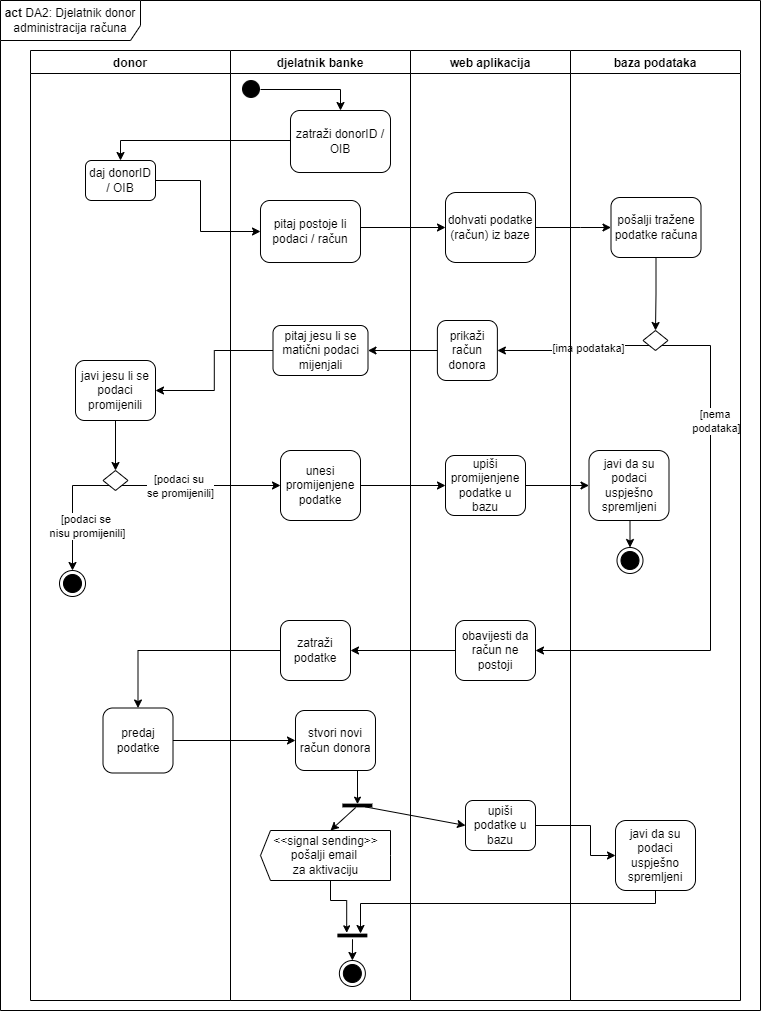
\includegraphics[scale=0.40]{slike/DA2 Djelatnik donor administracija racuna.png}
    	\centering
    	\caption{DA2 Djelatnik donor administracija računa}
    	\label{fig:da2}
    \end{figure}
    
    \par {Dijagram aktivnosti prikazan na slici 4.9 prikazuje upravljanje djelatnika banke donorovim računom. Djelatnik banke koristi donorov OIB kako bi utvrdio postoji li već račun koji odgovara tom donoru. Ako račun ne postoji, djelatnik banke kreira novi račun donora te sustav donoru šalje e-poruku za aktivaciju računa. Ukoliko račun postoji, a donorovi podaci su se promijenili, tada djelatnik banke ispravlja donorove podatke.}
			
%			\textbf{\textit{dio 2. revizije}}\\
			
%			 \textit{Potrebno je priložiti dijagram aktivnosti s pripadajućim opisom. Dijagram aktivnosti treba prikazivati značajan dio sustava.}
			
		\eject
		\section{Dijagram komponenti}
		
		\par{
		    Dijagram komponenti na slici 4.10 opisuje internu strukturu sustava, kako su komponente međusobno povezane te kako im se pristupa iz okoline.
		}
		\par{
		    Poslužitelj klijentske aplikacije poslužuje \textit{bundle.js} datoteku koja na klijentskom računalu pokreće klijentsku web aplikaciju, a ona generira sve potrebne HTML i CSS datoteke te JavaScript kod. 
		}
		\par{
		    Poslužiteljska aplikacija na krajnjim točkama (eng. \textit{endpoint}) API-ja (aplikacijsko-programskog sučelja) dočekuje zahtjeve klijentske aplikacije, obrađuje ih i vraća tražene podatke (ako oni postoje i ako klijentska aplikacija ima dopuštenje tražiti ih). API radi na REST principu, stoga ga nazivamo i REST API. REST API dio je Spring Boot kontrolera (eng. \textit{Controller}). Jednom kada neki kontroler primi zahtjev preko API-ja, on će odgovarajućem servisu proslijediti zahtjev, a od njega dobiti odgovor koji treba vratiti aplikaciji. Servisi (eng. \textit{service}) obrađuju zahtjeve koje im šalju kontroleri i dohvaćaju podatke iz repozitorija (eng. \textit{repository}), obrađuju te podatke te stvaraju odgovor koji vraćaju kontroleru. Repozitoriji podatke dobavljaju iz baze podataka pomoću SQL upita. Kako bi dobivene podatke mogli vratiti servisima koji će te podatke koristiti u obradi, koriste se modeli (eng. models), koji sadrže varijable koje odgovaraju određenim poljima iz baze podataka. Modeli su u pravilu jednostavni i sadrže varijable koje odgovaraju stupcima jedne tablice iz baze podataka. Kako nisu uvijek potrebni svi stupci neke tablice, podatci u prijenosu modeliraju se objektima za prijenos podataka (eng. \textit{DTO}), a moguće je da ti objekti ne sadrže sve varijable, već varijable koje odgovaraju samo nekim stupcima tablice.
		}
		\par{
		    PostgreSQL baza podataka na SQL upite vraća podatke iz baze podataka.
		}
		
		\begin{figure}[H]
            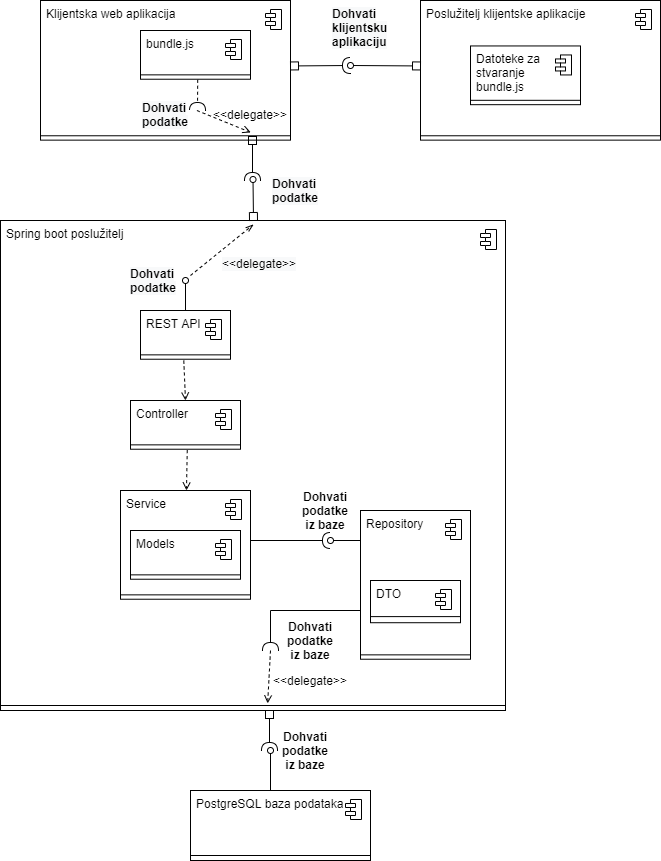
\includegraphics[scale=0.40]{slike/Dijagram komponenti 1_0.png}
        	\centering
        	\caption{Dijagram komponenti}
        	\label{fig:dk}
        \end{figure}
%			\textbf{\textit{dio 2. revizije}}\\
		
%			 \textit{Potrebno je priložiti dijagram komponenti s pripadajućim opisom. Dijagram komponenti treba prikazivati strukturu cijele aplikacije.}